\documentclass[a4-paper]{article}

\usepackage{amsmath}
\usepackage{amsfonts}
\usepackage{amssymb}
\usepackage[margin=2cm]{geometry}
\usepackage{setspace}
\onehalfspacing
\usepackage{parskip}
\usepackage{url}
%\usepackage{enumitem}
\usepackage{enumerate}
\usepackage{graphicx}
\usepackage{caption}
\usepackage{subcaption}
%\usepackage{listings}
\usepackage[all]{xy}
\usepackage{tikz}
\usetikzlibrary{bayesnet}

\newcommand{\vp}{\ensuremath{\varphi}}

\title{Derivation of Estimation and Maximization steps }
\begin{document}

\maketitle
\section{plate model}
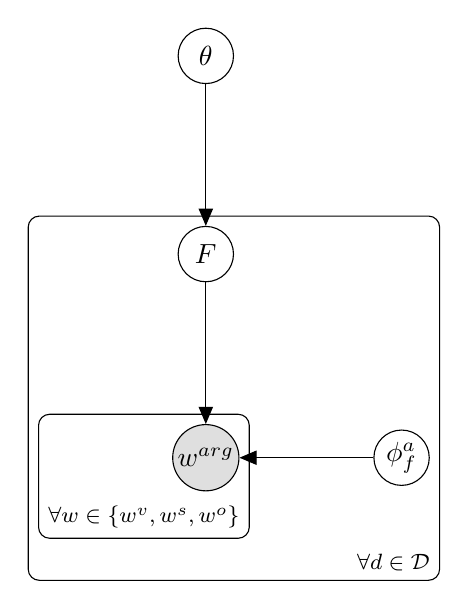
\begin{tikzpicture}[x=1.7cm,y=1.8cm]
    % Nodes
    \node[obs] (T) {$w^{arg}$} ; %
    \node[latent, above=of T] (F) {$F$} ; %
    \node[latent, above=of F] (theta) {$\theta$}; %
    \node[latent, right=of T] (phi) {$\phi^a_f$}; %
    \edge {theta} {F} ; %
    \edge {F} {T}
    \edge {phi} {T} ; %
    \plate {tuples} { (T) } {$\forall w \in \{w^v,w^s,w^o\}$}; %
    \plate {} { (tuples) (F) (phi)} {$\forall d \in \mathcal{D}$} ; %
\end{tikzpicture}
  
\section{table of variables}
\begin{tabular}{l l l }
  variable & description & range\\
  $f$ & frame & $ 1\leq f\leq F$\\
  $d=<v,s,o>_i$ & datapoints & $1\leq d\leq D$\\
  $\theta$ & probability distribution over $f$
  $\varphi_f^a$ & vector of probability distributions over words where $a\in\{v,s,o\}$ 
\end{tabular}

\section{E-step}

\[ P(f \mid d) = \mu(f) = \frac{P(d\mid f)P(d)}{\sum_{f=1}^F P(d\mid f) P(d)} \]\\
where:
\begin{align}
  P(d\mid f) &= \vp_f^v(v)\vp_f^s(s)\vp_f^s(s) \notag\\
  P(d) &= \sum_{f=1}^F\vp_f^v(v)\vp_f^s(s)\vp_f^s(s)\\
  P(f) &= \theta(f)
\end{align}

\section{M-step}

likelihood:
\begin{align}
  L(\theta,\vp)&=\sum_{d=1}^D\log\sum_{f=1}^FP(d,f\mid\theta\vp) \notag \\
  &=\sum_{d=1}^D\log\sum_{f=1}^FP(f)P(d\mid\theta\vp)
\end{align}

expectation of likelihood:
\begin{align}
  E_\mu[L] &= E_\mu[\sum_{d=1}^D\log P(d,f\mid\theta,\vp)]\notag\\
  &=\sum_{d=1}^DE_\mu[\log P(d,f\mid\theta,\vp)]\notag\\
  &=\sum_{d=1}^D\sum_{f=1}^F\mu_d(f)\log P(d,f\mid\theta,\vp)]
\end{align}
  

which gives us a decomposable maximization problem:
\begin{align}  
  &\arg\max_{\theta,\vp} \sum_{f=1}^F\sum_{d=1}^D \mu_d(f)\log P(f,d\mid\theta,\vp_f) = \notag\\
  &\arg\max_{\theta,\vp} \sum_{f=1}^F\sum_{d=1}^D \mu_d(f)\log(\theta(f)\vp^v_f(v)\vp^s_f(s)\vp^o_f(o))\notag\\
  &\arg\max_{\theta,\vp} \sum_{f=1}^F\sum_{d=1}^D \mu_d(f)(\theta(f)+\vp^v_f(v)+\vp^s_f(s)+\vp^o_f(o))
\end{align}

\subsection{$\arg\max_\theta$}
Since $\sum_{f=1}^F = 1$ we can use Lagrange function:
\begin{align}
  \arg\max_\theta L(\theta,\lambda) & = \sum_{f=1}^F\sum_{d=1}^D \mu_d(f)\log(\theta(f)+\lambda(\sum_{f=1}^F\theta(f) -1 )) \Rightarrow \notag\\
  L(\theta,\lambda)\frac{df}{d\theta(f)} & = \frac{\sum_{d=1}^D\mu_d(f)}{\theta(f)}-\lambda = 0 \Rightarrow \notag\\
  \theta(f)(\lambda) &= \frac{\sum_{d=1}^D\mu_d(f)}{\lambda}\quad\&\quad \sum_{f=1}^F\theta(f)(\lambda*) = 1 \Rightarrow \notag\\
  \frac{\sum_{d=1}^D\sum_{f=1}^F\mu_d(f)}{\lambda *} &= 1 \rightarrow \lambda *=\sum_{d=1}^D\sum_{f=1}^F\mu_d(f)  \Rightarrow \notag\\
    & \text{replacing } \lambda \text{ for } \lambda* \Rightarrow \notag\\
    \theta(f) &= \frac{\sum_{d=1}^D\mu_d(f)}{\sum_{d=1}^D\sum_{f=1}^F\mu_d(f)} \notag\\
\end{align}

\subsection{$\arg\max_\vp$}
Since $\sum_{w=1}^V = 1$ we can use Lagrange function:
\begin{align}
  \arg\max_{\vp^a_f} L(\vp^a_f,\lambda) & = \sum_{f=1}^F\sum_{d=1}^D \mu_d(f)\log(\vp^a_f(a)+\lambda(\sum_{w=1}^V\vp_a^f(a) -1 )) \Rightarrow \notag\\
  L(\theta,\lambda)\frac{da}{d\vp_f^a(a)} & = \frac{\sum_{d=1}^D\mu_d(f)}{\vp_f^a(a)}-\lambda = 0 \Rightarrow \notag\\
  \dots \notag\\
  \vp_f^a(a) &= \sum^D_{d=1}\mu_d(f)*C(w,a) \notag \\
\end{align}
(where $C(w,a)$ is the count of $w$ appearing as $a$).\\



\end{document}
